% !TeX spellcheck = it_IT
\newpage
\section{Agenti risolutori di problemi}
Gli agenti risolutori di problemi adottano il paradigma della risoluzione di problemi come \textbf{ricerca} in uno \textbf{spazio di stati}. Sono agenti con \textbf{modello} (storia percezioni e stati) che adottano una rappresentazione \textbf{atomica} degli stati.\\
Sono particolari gli agenti con \textbf{obiettivo} che pianificano l'intera sequenza di mosse prima di agire.

\subsection{Processo di risoluzione}
I passi da seguire sono i seguenti:
\begin{enumerate}
	\item \textbf{Determinazione di un obiettivo}, ovvero un insieme di stati in cui l'obiettivo è soddisfatto
	\item \textbf{Formulazione} del problema tramite la rappresentazione degli stati e delle azioni
	\item Determinazione della \textbf{soluzione} mediante la ricerca
	\item \textbf{Esecuzione} del piano
\end{enumerate}

\begin{example}[Viaggio con mappa]
	Supponiamo di voler fare un viaggio. Il processo di risoluzione sarebbe il seguente:
	\begin{enumerate}
		\item Raggiungere Bucarest
		\item \begin{itemize}
			\item Azioni: guidare da una città all'altra
			\item Stato: città su mappa
		\end{itemize}
	\end{enumerate}
\end{example}

\subsection{Assunzioni}
Assumiamo che l'ambiente in questione sia \textbf{statico}, \textbf{osservabile}, \textbf{discreto} e \textbf{deterministico} (assumiamo un mondo ideale).

\subsection{Formulazione del problema}
Un problema può essere definito formalmente mediante 5 componenti:
\begin{enumerate}
	\item \textbf{Stato iniziale}
	\item \textbf{Azioni} possibili
	\item \textbf{Modello di transizione}: $ris: stato \times azione \to stato$, uno stato \emph{successore} $ris(s,a)=s'$
	\item \textbf{Test obiettivo} per capire tramite un insieme di stati obiettivo se il goal è raggiunto $test: stato \to \{true,false\}$
	\item \textbf{Costo del cammino}: composto dalla somma dei costi delle azioni, dove un passo ha costo $c(s,a,s')$. Un passo non ha mai costo negativo.
\end{enumerate}
I punti 1, 2 e 3 definiscono implicitamente lo \textbf{spazio degli stati}. Definirlo esplicitamente può essere molto costoso.

\subsection{Algoritmo di ricerca}
Gli algoritmi di ricerca prendono in input un problema e restituiscono un \textbf{cammino soluzione}.\\
Dobbiamo misurare le \textbf{prestazioni}: trova una soluzione? Quanto costa trovarla? Quanto è efficiente?
\begin{equation*}
	costo\_totale=costo\_ricerca+costo\_cammino\_sol
\end{equation*}

\begin{example}[Arrivare a Bucarest]
	Partiamo con la formulazione del problema:
	\begin{enumerate}
		\item \textbf{Stato iniziale}: la città di partenza, ovvero Arad
		\item \textbf{Azioni}: spostarsi in una città collegata vicina
		\begin{lstlisting}
			Azioni(In(Arad))={Go(Sibiu),Go(Zerind),...}
		\end{lstlisting}
		\item \textbf{Modello di transizione}: 
		\begin{lstlisting}
			Risultato(In(Arad), Go(Sibiu)) = In(Sibiu)
		\end{lstlisting}
		\item \textbf{Test obiettivo}:
		\begin{lstlisting}
			{In(Bucarest)}
		\end{lstlisting}
		\item \textbf{Costo del cammino}: somma delle lunghezze delle strade
	\end{enumerate}
	In questo esempio lo spazio degli stati coincide con la rete dei collegamenti tra le città.
	\begin{center}
		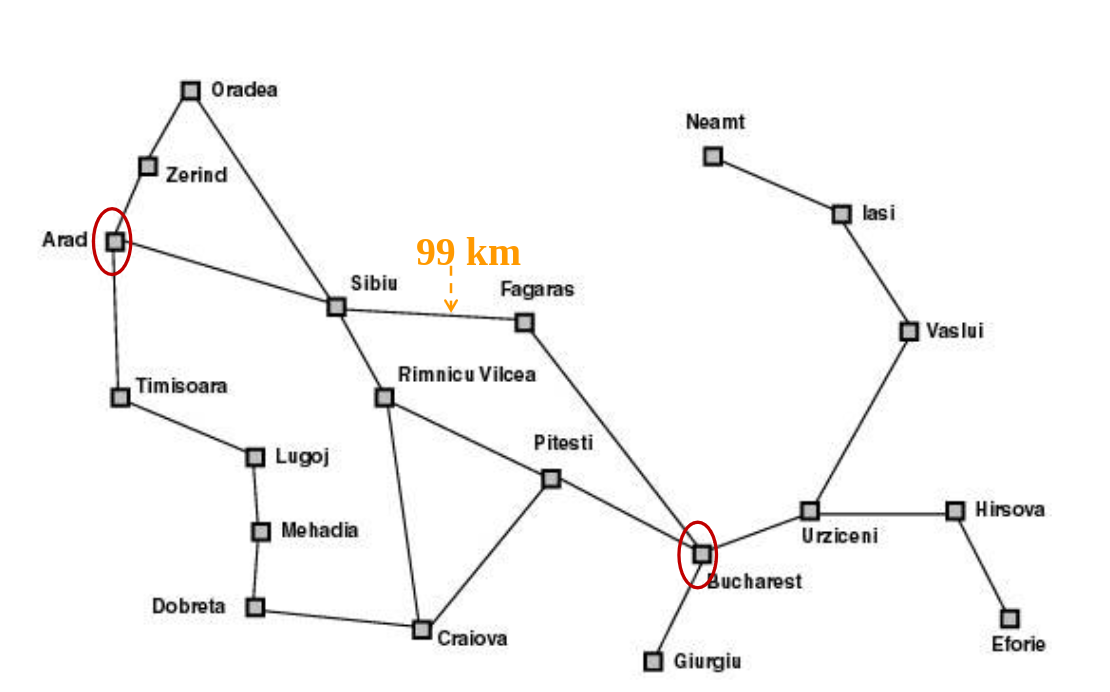
\includegraphics[scale=0.2]{images/bucarest_example.png}
	\end{center}
\end{example}

\begin{example}[Puzzle dell'8]
	Partiamo con la formulazione del problema:
	\begin{enumerate}
		\item \textbf{Stati}: tutte le possibili configurazioni della scacchiera
		\item \textbf{Stato iniziale}: una configurazione tra quelle possibili
		\item \textbf{Obiettivo}: una configurazione del tipo
		\begin{center}
			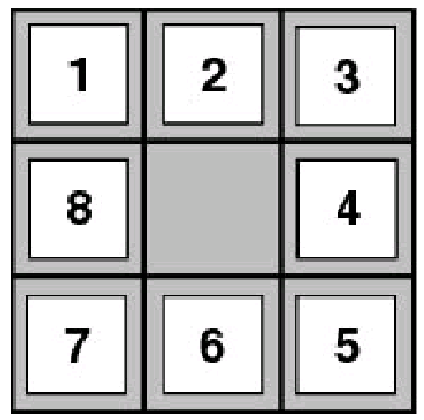
\includegraphics[scale=0.2]{images/8_puzzle_win.png}
		\end{center}
		\item \textbf{Azioni}: le mosse della casella vuota
		\item \textbf{Costo cammino}: ogni passo costa 1
	\end{enumerate}
	In questo esempio lo spazio degli stati è un grafo con possibili cicli (ci possiamo ritrovare in configurazioni già viste). Il problema è NP-completo: per 8 tasselli ci sono $\frac{9!}{2}=181.000$ stati.
\end{example}

\begin{example}[8 regine]
	Supponiamo di dover collocare 8 regine su una scacchiera in modo tale che nessuna regina sia attaccata da altre.
	\begin{enumerate}
		\item \textbf{Stati}: tutte le possibili configurazioni della scacchiera con 0-8 regine
		\item \textbf{Goal test}: avere 8 regine sulla scacchiera, di cui nessuna è attaccata
		\item \textbf{Azioni}: aggiungi una regina
	\end{enumerate}
	In questo esempio lo spazio degli stati sono le possibili scacchiere, ovvero $64 \times 63 \times \ldots \times 57 \simeq 1.8 \times 10^{14}$.\\
	Proviamo ad utilizzare una formulazione diversa:
	\begin{enumerate}
		\item \textbf{Stati}: tutte le possibili configurazioni della scacchiera in cui \emph{nessuna regina è minacciata}
		\item \textbf{Goal test}: avere 8 regine sulla scacchiera, di cui nessuna è attaccata
		\item \textbf{Azioni}: aggiungere una regina nella colonna vuota più a destra ancora libera in modo che non sia minacciata
	\end{enumerate}
	Lo spazio degli stati passa a $2057$, anche se comunque rimane esponenziale per $k$ regine.\\
	Vediamo infine un'ultima formulazione:
	\begin{enumerate}
		\item \textbf{Stati}: scacchiere con 8 regine, una per colonna
		\item \textbf{Goal test}: nessuna delle regine già presenti è attaccata
		\item \textbf{Azioni}: sposta una regina nella colonna se minacciata
		\item \textbf{Costo cammino}: zero
	\end{enumerate}
	Qui lo spazio degli stati è di qualche decina di milione.\\
	Capiamo quindi che formulazioni diverse del problema portano a spazi di stati di dimensioni diverse.
\end{example}

\begin{example}[Dimostrazione di teoremi]
	Dato un insieme di premesse:
	\begin{equation}
		\{s, t, q \Rightarrow p, r \Rightarrow p, v \Rightarrow q, t \Rightarrow r, s \Rightarrow v\}
	\end{equation}
	dimostrare una proposizione $p$ utilizzando solamente la regola di inferenza \emph{Modus Ponens}:
	\begin{equation*}
		(p \wedge p\Rightarrow q) \Rightarrow q
	\end{equation*}
	Scriviamo la formulazione del problema:
	\begin{itemize}
		\item \textbf{Stati}: insieme di proposizioni
		\item \textbf{Stato iniziale}: le premesse
		\item \textbf{Stato obiettivo}: un insieme di proposizioni contenente il teorema da dimostrare
		\item \textbf{Operatori}: l'applicazione del Modus Ponens
	\end{itemize}
	Lo spazio degli stati è quindi il seguente:
	\begin{center}
		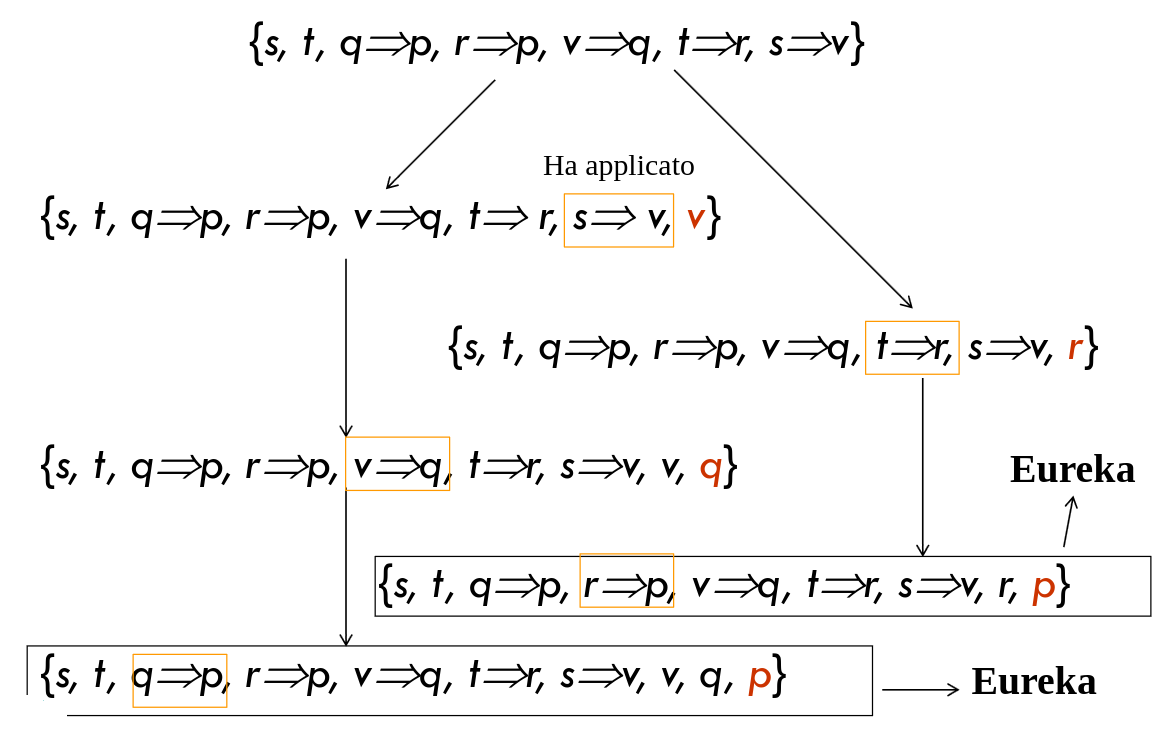
\includegraphics[scale=0.3]{images/dimostrazione_teoremi.png}
	\end{center}
\end{example}

\subsection{Ricerca della soluzione}
La ricerca della soluzione consiste nella generazione di un \textbf{albero di ricerca} a partire dalle possibili sequenze di azioni che si sovrappone allo spazio degli stati.\\
Ad esempio per il caso di Bucarest:
\begin{center}
	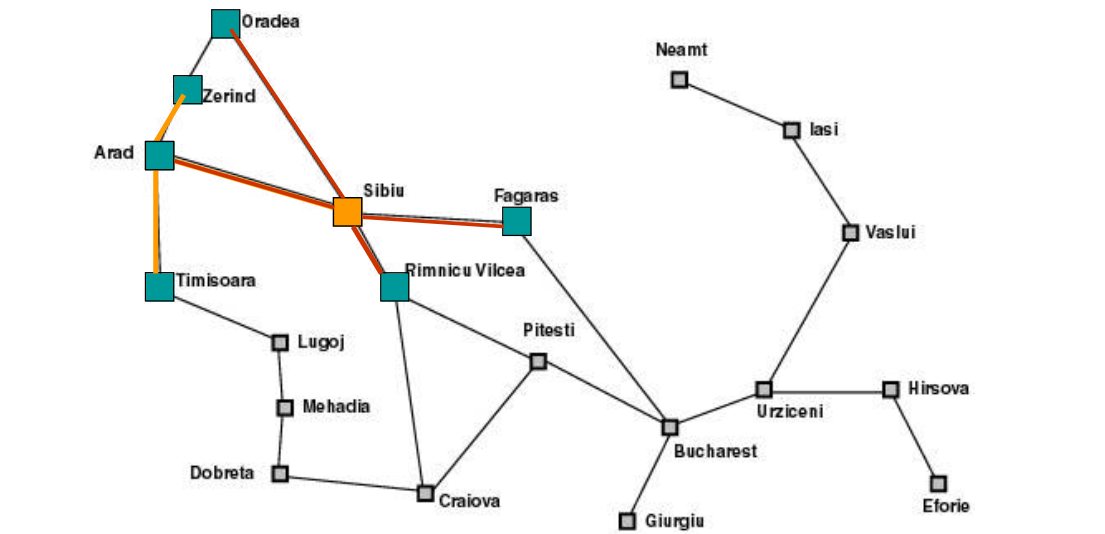
\includegraphics[scale=0.3]{images/bucarest_tree.png}
\end{center}
Espandiamo ogni nodo con i suoi possibili successori (frontiera).
\begin{observation}
	Si noti che un nodo dell'albero è diverso da uno stato. Infatti possono esitere nodi dell'albero di ricerca con lo stesso stato (si può tornare indietro).
\end{observation}

\subsection{Ricerca in ampiezza (BF)}
O come esplorare il grafo dello spazio degli stati a livelli progressivi di stessa profondità.
\begin{lstlisting}
	function Ricerca-Ampiezza (problema)
		return soluzione oppure fallimento
		nodo = un nodo con stato il problema.stati-iniziale e costo-di-cammino=0
		if problema.Test-Obiettivo(nodo.Stato) then return Soluzion(nodo)
		frontiera = una coda FIFO con nodo come unico elemento
		loop do
			if(Vuota?(frontiera)) then return fallimento
			nodo = POP(frontiera)
			for each azione in problema.Azioni(nodo.Stato) do
				figlio = Nodo-Figlio(problema, nodo, azione) [costruttore: vedi AIMA]
				if Problema.TestObiettivo(figlio.Stato) then return Soluzione(figlio)
				frontiera = Inserisci(figlio, frontiera) /* frontiera gestita come coda FIFO
\end{lstlisting}
\begin{note}
	Nota che in questa versione i nodo.stato sono goal-tested al momento in cui sono generati, anticipato→ più efficiente, si ferma appena trova goal prima di espandere.
\end{note}
Una versione aggiornata dove evitiamo di espandere (nodi con) stati già esplorati:
\begin{lstlisting}
	function Ricerca-Ampiezza (problema)
		return soluzione oppure fallimento
		nodo = un nodo con stato il problema.stati-iniziale e costo-di-cammino=0
		if problema.Test-Obiettivo(nodo.Stato) then return Soluzion(nodo)
		frontiera = una coda FIFO con nodo come unico elemento
		esplorati = indieme vuoto //aggiunto per gestire gli stati ripetuti
		loop do
			if(Vuota?(frontiera)) then return fallimento
			nodo = POP(frontiera) // aggiungi nodo.Stato a esplorati
			for each azione in problema.Azioni(nodo.Stato) do
				figlio = Nodo-Figlio(problema, nodo, azione) [costruttore: vedi AIMA]
				if figlio.Stato non e in esplorati e non e in frontiera then // aggiunto check per vedere se e in frontiera
				frontiera = Inserisci(figlio, frontiera) /* frontiera gestita come coda FIFO
\end{lstlisting}
Abbiamo aggiunto \textbf{esplorati = insieme vuoto} e \textbf{if figlio.Stato non è in esplorati e non è in frontiera then} 
per gestire gli stati ripetuti.\\\\
Ora sempre lo stesso codice in uno script python:
\begin{lstlisting}
	def breadth_first_search(problem): # """Ricerca-grafo in ampiezza"""
		explored = [] # insieme degli stati gia visitati (implementato come una lista)
		node = Node(problem.initial_state) # il costo del cammino e inizializzato nel
		costruttore del nodo
		if problem.goal_test(node.state):
			return node.solution(explored_set = explored)
		frontier = FIFOQueue() # la frontiera e' una coda FIFO
		frontier.insert(node)
		while not frontier.isempty(): # seleziona il nodo per l'espansione
			node = frontier.pop()
			explored.append(node.state) # inserisce il nodo nell'insieme dei nodi esplorati
			for action in problem.actions(node.state):
				child_node = node.child_node(problem,action)
				if (child_node.state not in explored) and (not frontier.contains_state(child_node.state)):
					if problem.goal_test(child_node.state):
						return child_node.solution(explored_set = explored)
				# se lo stato non e' uno stato obiettivo allora inserisci il nodo nella frontiera
				frontier.insert(child_node)
		return None # in questo caso ritorna con fallimento
\end{lstlisting}

\subsubsection*{Analisi complessità spazio-temporale (BF)}
Inanzitutto assumiamo che:
\begin{itemize}
	\item \textbf{b} = fatto di ramificazione (\textbf{b}ranching)
	\item \textbf{d} = profondità del nodo obiettivo piu superficiale (\textbf{d}epth) 
	\item \textbf{m} = lunghezza massima dei cammini nello spazio degli stati (\textbf{m}ax)
\end{itemize}
La strategia ottimale è se gli operatori hanno tutti lo stesso costo k cioè $g(n) = k \cdot depth(n)$ dove $g(n)$ è il costo del 
cammino per arrivare a n.\\
\textbf{La complessità nel tempo} (nodi generati):
$$T(b, d) = 1 + b + b^2 + \dots + b^d \to O(b?d) \:\: \text{b figli per ogni nodo}$$
\begin{note}
	Riflettere che il numero nodi cresce exp., non assumiamo di conoscere già il
	grafo ne una notazione di linearità nel numero nodi . Questo è tipico dei problemi in
	AI (pensate a quelli generati per le configurazioni dei giochi, con rappresentazione
	implicita dello spazio stati, non esplicitamente/staticamente in spazi enormi).
\end{note}
\textbf{Complessità nello spazio} (nodi in memoria): $O(b^d)$

\begin{example}
	b=10, 1 milione nodi al sec generati; 1 nodo occupa 1000 byte
	% TODO aggiungi immagine tempo e memoria per questo esempio.
\end{example}

\subsection{Ricerca in profondità (DF)}
Viene implementata da una coda che mette i succerrosi in testa alla lista (LIFO, pila o stack). Notare
come cancelli rami completamente esplorati ma tenga tutti i fratelli del path corrente: memoria solo $b \times m$

\subsubsection*{Analisi}
\textbf{Versione su albero}.\\\\
Se $m \to$ lungehzza massima dei cammini nello spazio degli stati e $b \to$ fattore di diramazione.
\textbf{Abbiamo che tempo}: $O(b^m)$ [che può essere $> O(b^d)$].
\textbf{Occupazione memoria}: $bm$ [frontiera sul cammino].

% TODO Finisci la slide
\textbf{Versione su grafo}
In caso di DF con visita grafo si perderebbe i vantaggi di memoria. la memoria torna da
$bm$ a tutti i possibili stati (potenzialmente, caso pessimo, esponenziale come BF*) (per mantenere la lista
dei visitati/esplorati), ma così DF diviene \textbf{completa} in spazi degli stati finiti (tutti 
i nodi verranno espansi nel caso pessimo).

\begin{lstlisting}
	function Ricerca-DF-A (problema)
		returns soluzione oppure fallimento
		return Ricerca-DF-ricorsiva(CreaNodo(problema.Stato-iniziale), problema)
		
	function Ricerca-DF-ricorsiva(nodo, problema)
		returns soluzione oppure fallimento
		if problema.TestObiettivo(nodo.Stato) then return Soluzione(nodo)
		else
		for each azione in problema.Azioni(nodo.Stato) do
			figlio = Nodo-Figlio(problema, nodo, azione)
			risultato = Ricerca-DF-ricorsiva(figlio, problema)
			if risultato != fallimento then return risultato
		return fallimento
\end{lstlisting}
Versione scritta in python:
\begin{lstlisting}
	def recursive_depth_first_search(problem, node):
		"""Ricerca in profondita' ricorsiva """
		# controlla se lo stato del nodo e' uno stato obiettivo
		if problem.goal_test(node.state):
			return node.solution()
		# in caso contrario continua
		for action in problem.actions(node.state):
			child_node = node.child_node(problem, action)
			result = recursive_depth_first_search(problem, child_node)
			if result is not None:
				return result
		return None #con fallimento
\end{lstlisting}

\subsection{Approfondimento iterativo (ID)}
Si prova DF (DL) con limite di profondità 0, poi 1, poi 2, poi 3 ... fino
a trovare la soluzione.
% TODO inserire immagine

Miglior comprosmesso tra BF e DF.
$$BF: b + b^2 + \dots + b^{d-1} + b^d \:\:\: con b=10 e d=5$$
$$10 + 100 + 1000 + 10.000 + 100.000 = 111.110$$
ID: i nodi dell'ultimo livello generati una volta, quelli del penultimo 2, quelli
del terzultimo 3 ... quelli del primo d volte.
$$ID: (d)b + (d-1)b^2 + \dots + 3b^{d-2} + 2b^{d-1} + 1b^d$$
$$= 50 + 400 + 3000 + 20.000 + 100.000 = 123.450$$
\textbf{Complessita tempo}: $O(b^d)$ (se esiste soluzione)
\textbf{Spazio}: $O(bd)$ (se esiste soluzione) versus $O(b^d)$ della BF.

\subsection{Ridondanze}
Su spazi di stati a grafo si possono generare piu volte gli stesso nodi 
(o meglio nodi con stesso stato) nella ricerca, \textbf{anche in assenza di cicli}
(cammini ridondanti).\\\\
Se vediamo per esempio il caso di ridondance nelle griglie spesso si vanno a visitare stati
già visitati questa operazione fa compiere lavoro inutile. Come evitarlo?\\\\
Ricordare gli stati già visitati occupa spazio (es. lista \textbf{esplorati} in visita a grafo) ma ci consente di evitare di visitarli di nuovo.
Gli algoritmi che dimenticano la propria storia sono desinati a ripeterlo!
Abbiamo tre soluzioni, in ordine crescente di costo e di efficacia:
\begin{itemize}
	\item Non tornare nello stato da cui si proviene: si elimina il
	genitore dai nodi successori (non evita i cammini ridondanti).
	\item Non creare cammini con cicli: si controlla che i successori
	non siano antenati del nodo corrente (detto per la DF).
	\item Non generare nodi con stati già visitati/esplorati: ogni
	nodo visitato deve essere tenuto in memoria per una
	complessità O(s) dove s è il numero di stati possibili (e.g.
	hash table per accesso efficiente).
\end{itemize}
Ricordare che il costo può essere alto: in caso di DF (profon.) la
memoria torna da bm a tutti gli stati, ma diviene una ricerca
completa (per spazi finiti). Ma in molti casi gli stati crescono exp.
(gioco otto, scacchi, \dots)

\subsection{Ricerca di costo uniforme (UC)}
Generalizzazione della ricerca in ampiezza (costi diversi tra passi): si sceglie il
nodo di costo minore sulla frontiera (si intende il costo $g(n)$ del cammino), si espande sui 
contorni di \textbf{uguale (o meglio uniforme) costo (e.g. in km)} invece che sui
contorni di uguale profondità (BF).
%% TODO aggiungi foto
Implementata da una coda ordinata per costo cammino crescente (in cima i nodi di costo minore).
Codice di ricerca UC su albero:
\begin{lstlisting}
	function Ricerca-UC-A (problema)
		returns soluzione oppure fallimento
		nodo = un nodo con stato il problema.stato-iniziale e costo-di-cammino=0
		frontiera = una coda con priorita con nodo come unico elemento
		loop do
			if Vuota?(frontiera) then return fallimento
			nodo = POP(frontiera)
			// Posticipato* per vedere il costo minore su g (diverso da BF, ma tipico per coda priorita)
			if problema.TestObiettivo(nodo.Stato) then return Soluzione(nodo)
			for each azione in problema.Azioni(nodo.Stato) do
				figlio = Nodo-Figlio(problema, nodo, azione)
				frontiera = Inserisci(figlio, frontiera) /* in coda con priorita
	end
\end{lstlisting}
Codice di ricerca UC su grafo:
\begin{lstlisting}
	function Ricerca-UC-G (problema)
		returns soluzione oppure fallimento
		nodo = un nodo con stato il problema.stato-iniziale e costo-di-cammino=0
		frontiera = una coda con priorita con nodo come unico elemento
		esplorati = insieme vuoto
		loop do
			if Vuota?(frontiera) then return fallimento
			nodo = POP(frontiera);
			// posticipato per vedere il costo minore
			if problema.TestObiettivo(nodo.Stato) then return Soluzione(nodo)
			aggiungi nodo.Stato a esplorati
			for each azione in problema.Azioni(nodo.Stato) do
				figlio = Nodo-Figlio(problema, nodo, azione)
				if figlio.Stato non e in esplorati e non e in frontiera then
					frontiera = Inserisci(figlio, frontiera) /* in coda con priorita
				else if figlio.Stato e in frontiera con Costo-cammino piu alto then // costo cammino piu alto g
					sostituisci quel nodo frontiera con figlio
\end{lstlisting}

\subsubsection{Analisi}
Ottimalità e completezza garantite purchè il costo degli archi sia maggiore di $\epsilon > 0$.
Appunto $C^*$ come il costo della soluzione ottima, $\lfloor C^*/\epsilon \rfloor$ è il numero 
di mosse nel caso peggiore, arrotondato per difetto (e.g. attratto ad andare versio tante bassa)\\\\
\textbf{Complessità}: $O(b^{1+\lfloor C^*/\epsilon}\rfloor)$
\begin{note}
	Quando ogni azione ha lo stesso costo UC somiglia a BF ma complessità $O(b^{1+d})$
\end{note}
Causa esame ed arresto posticipato, solo dopo aver espando frontiera, oltre la profondità del goal.
